\documentclass[12pt, a4paper]{article}

% Paquetes básicos
\usepackage[utf8]{inputenc} % Codificación de caracteres
\usepackage[spanish]{babel} % Idioma 
\usepackage{tikz}
\usepackage{subcaption}
\usepackage{setspace} % Para configurar el interlineado
\usepackage{geometry} % Configuración de márgenes
\usepackage{hyperref} % Para enlaces a repositorios y correos
\usepackage{amsmath}
\usepackage[font=small,labelfont=bf]{caption}
% Configuración de márgenes estándar
\geometry{top=2.5cm, bottom=2.5cm, left=3cm, right=3cm}

% Aplicar interlineado sencillo en todo el documento
\singlespacing

\begin{document}

% -------------------------------------------------------------
% PORTADA
% -------------------------------------------------------------
\begin{titlepage}
    \centering
    \vspace*{2cm}
    
    {\Huge \textbf{Producción de monopolos magnéticos en el LHC}}\\[2cm]
    
    {\Large \textbf{Alumno:}}\\
    Alonso Rodríguez Calleja\\
    \href{mailto:calleja4@alumni.uv.es}{calleja4@alumni.uv.es}\\[1.5cm]
    
    {\Large \textbf{Supervisora: }}\\
    Vasiliki Mitsou\\
    \href{mailto:Vasiliki.Mitsou@ific.uv.es}{Vasiliki.Mitsou@ific.uv.es}\\[2cm]
    
    \vfill
    
    % Información institucional opcional para darle buen formato
    {\Large  Estancia de Investigación}\\
    {\normalsize Máster en Física}\\
    {\normalsize Universitat de València}\\[1cm]
    
    {\normalsize \today}
\end{titlepage}

% Reiniciar contador de páginas después de la portada
\setcounter{page}{2}

% -------------------------------------------------------------
% SECCIÓN 1: Descripción del grupo
% -------------------------------------------------------------
\section{Grupo AITANA}

El grupo de investigación multidisciplinar AITANA, perteneciente al Instituto de Física Corpuscular (IFIC), se encuentra instalado en el Parc Científic de la Universitat de València (Paterna). Sus líneas principales de investigación abarcan los experimentos en el LHC y futuros colisionadores, la física de axiones y ondas gravitacionales, así como las aplicaciones de aceleradores en física médica.

En particular, esta estancia se ha desarrollado dentro de su participación en MOEDAL (Monopole and Exotics Detector at the LHC), el séptimo experimento del Gran Colisionador de Hadrones (LHC). El objetivo principal de este proyecto es buscar evidencias de nueva física complementando a ATLAS, CMS y LHCb. Para ello, el detector rastrea partículas masivas, estables, altamente no relativistas y fuertemente ionizantes, enfocándose especialmente en la búsqueda de monopolos magnéticos y diones \cite{doi:10.1126/science.165.3895.757} empleando las altas energías del LHC.

Cabe destacar que el grupo del IFIC, unido de forma oficial a \textsc{MoEDAL} en el año 2012, representa la única participación española en todo el experimento \textsc{MoEDAL}.
% -------------------------------------------------------------
% SECCIÓN 2: Descripción de la actividad
% -------------------------------------------------------------
\section{Descripción de la actividad}
% Debe incluir introducción, desarrollo y resultados.
\subsection{Introducción}

Desde las primeras clases del grado, se nos ha dicho que los monopolos magnéticos no existen. Esto se debe a que la Electrodinámica Clásica establece que:
\begin{equation}
    \boldsymbol{\nabla}\cdot \boldsymbol{B}=0\ ,
\end{equation}
invalidando así la presencia de cargas magnéticas aisladas. Sin embargo, durante el desarrollo de la Mecánica Cuántica, el rol del potencial vector $\boldsymbol{A}$ se vio extendido a más allá de ser una herramienta matemática, apareciendo así dentro de las fases cuánticas. Debido a esto, Dirac demostró que la mera existencia de una única carga magnética $g$ bastaba para que la carga eléctrica $e$ estuviese cuantizada. Esto queda establecido según la \textit{Condición de Cuantización de Dirac} (DQC) \cite{Dirac1931}:
\begin{equation}
    ge=2\pi\hbar c\cdot n, \quad n\in \mathbf{N}\ .
\end{equation}
Por tanto, los monopolos magnéticos ofrecen un mecanismo para explicar la cuantización de la carga, que es un fenómeno ampliamente observado en la naturaleza.

Unos años después, los físicos Gerard 't Hooft y Alexander Polyakov \cite{Polyakov1974,tHooft1974} demostraron que los monopolos magnéticos no son un simple artilugio matemático. Por el contrario, demostraron que son predicciones de ciertas teorías gauge no abelianas que satisfacen determinadas condiciones topológicas. Sorprendentemente, estas condiciones topológicas, son satisfechas por el propio Modelo Estándar (SM). De esta manera, los monopolos magnéticos se convierten en una predicción de la teoría más exitosa de la historia de la Física.

\subsubsection{Principales retos en la física de monopolos}
A pesar de que los monopolos son predicciones del SM, su posible existencia plantea una serie de desafíos. Por un lado desde el punto de vista teórico:
\begin{itemize}
    \item Los monopolos aparecen de manera natural como soluciones clásicas de las ecuaciones de campo (solitones topológicos). El tratamiento cuántico, por consiguiente, precisa cuantizar de manera consistente el monopolo junto con la electrodinámica cuántica, lo cual resulta un problema no trivial.
    \item La DQC define una constante de estructura fina propia del monopolo magnético $\alpha_g$, que está relacionada con la del electrón ($\alpha_e$) mediante la expresión $\frac{\alpha_g}{\alpha_e}\approx 68$.
    Por tanto, cualquier cálculo perturbativo estaría teóricamente invalidado debido a este alto valor.
\end{itemize}
Mientras que desde el punto de vista experimental:
\begin{itemize}
    \item Las predicciones teóricas conllevan un alto valor para la masa del monopolo \cite{2016,MoEDAL2017,mitsou2026magneticmonopolesdirac}, de aproximadamente $\mathcal{O}(1-10)$ TeV. Esta enorme masa dificulta en gran medida la producción de monopolos en los aceleradores.
    \item Un monopolo magnético de carga $g_D \equiv 2\pi\hbar c/e$ se comporta al atravesar la materia de forma equivalente a un átomo de $Z \approx 69$. Debido a esto, pierde energía 4700 veces más rápido que un electrón, condicionando enormemente toda la estructura tecnológica necesaria para su detección.
\end{itemize}
\subsection{Simulaciones en MadGraph}

Durante el desarrollo de esta investigación, la herramienta de trabajo computacional ha sido el software \texttt{MadGraph5\textunderscore aMC@NLO} (o simplemente \texttt{MadGraph}) \cite{Alwall_2014}. Este programa es un generador de eventos que basa su funcionamiento en métodos de Monte Carlo.

En el contexto concreto del experimento \textsc{MoEDAL}, el uso de \texttt{MadGraph} cobra una especial relevancia por dos motivos fundamentales: primero, permite simular escenarios personalizados o exóticos, obteniendo así cálculos teóricos que sirven para buscar nueva física en los experimentos; y segundo, pese a que \texttt{MadGraph} está diseñado para calcular la física en el instante exacto de la colisión, el programa goza con una amplia compatibilidad con otros programas (como \texttt{Pythia} o \texttt{Geant4}) , que toman relevo para simular el resto de la cascada de partículas  y cómo estas interactúan con los sensores del detector
\subsubsection{Breve descripción de su funcionamiento}
Para un proceso de scattering $i\to f$, la sección eficaz total se puede expresar mediante la siguiente estructura general:
\begin{equation}
    \sigma(i\to f)=\mathcal C\int d\Phi\ |\mathcal M|^2\ .
\end{equation}
Donde $d\Phi$ representa la medida del espacio de fases, $\mathcal{C}$ es un coeficiente que incorpora la dependencia cinemática y $\mathcal{M}$ representa la amplitud de transición cuántica de dicho proceso, determinada por una suma infinita de diagramas de Feynman, por lo que es necesario truncar dicha serie a un orden fijo de aproximación para realizar predicciones.
El razonamiento algorítmico que sigue \texttt{MadGraph} se desglosa en dos fases:
\begin{enumerate}
    \item \textbf{Configuración y generación de código}: Se comienza definiendo el modelo teórico, las partículas involucradas y los órdenes de interacción. Después se construyen todos los diagramas de Feynman al orden especifico, para después construir la amplitud de probabilidad. Posteriormente se realiza álgebra de color y de Lorentz, así como las pertinentes simplificaciones. Finalmente, se genera el código para la generación de eventos.
    \item \textbf{Generación de eventos}: Importando el código anterior, así como los valores numéricos de las constantes requeridas (modificables dentro de archivos \texttt{run\textunderscore cards} y \texttt{param\textunderscore cards}). Luego, se genera el espacio de fases y se evalúa el cuadrado de la amplitud de probabilidad. Por último, se integra usando métodos Monte Carlo, exportando así un archivo \texttt{.LHE}.
\end{enumerate}

\subsubsection{Aplicación a la física de monopolos}
En el contexto de los colisionadores de partículas, los principales mecanismos teóricos para la producción de monopolos magnéticos son mediante procesos de Drell-Yan (DY), fusión de fotones y por efecto Schwinger. Los dos primeros procesos son de naturaleza perturbativa y están esquematizados en la Figura \ref{Feynmandiag}. Por tanto, para que el cálculo de estos diagramas de Feynman tenga un sentido físico, es preciso trabajar cerca del umbral de producción del par. En este régimen, la constante de acoplamiento efectiva se modifica como sigue \cite{Baines2018}:
\begin{equation}\label{gbeta}
    g\mapsto g\hat\beta\equiv g\sqrt{1-\frac{4M^2}{s}}\ .
\end{equation}
De esta manera, se cumple que $g\hat{\beta} \ll 1$, lo que permite aplicar la teoría de perturbaciones. En particular, esta investigación se centrará de forma específica en el canal de producción Drell-Yan. Por otro lado, la producción mediante el efecto Schwinger presenta un escenario no perturbativo que, a diferencia de su análogo para campos eléctricos, presenta un campo crítico $|\boldsymbol B| \sim 10^{16}$ T, un valor que sí es posible alcanzar tecnológicamente en colisiones actuales \cite{MoEDAL2022}.


\begin{figure}[ht!]
    \centering


\tikzset{every picture/.style={line width=0.75pt}} %set default line width to 0.75pt        

\begin{tikzpicture}[scale=0.8,x=0.75pt,y=0.75pt,yscale=-1,xscale=1]
%uncomment if require: \path (0,300); %set diagram left start at 0, and has height of 300

%Straight Lines [id:da3283572493917589] 
\draw    (98.2,69.6) -- (137.63,130.5) ;
\draw [shift={(137.63,130.5)}, rotate = 57.08] [color={rgb, 255:red, 0; green, 0; blue, 0 }  ][fill={rgb, 255:red, 0; green, 0; blue, 0 }  ][line width=0.75]      (0, 0) circle [x radius= 2.68, y radius= 2.68]   ;
\draw [shift={(119.98,103.24)}, rotate = 237.08] [fill={rgb, 255:red, 0; green, 0; blue, 0 }  ][line width=0.08]  [draw opacity=0] (7.14,-3.43) -- (0,0) -- (7.14,3.43) -- cycle    ;
%Straight Lines [id:da3276659901466582] 
\draw    (137.63,130.5) -- (98.2,191.4) ;
\draw [shift={(115.85,164.14)}, rotate = 302.92] [fill={rgb, 255:red, 0; green, 0; blue, 0 }  ][line width=0.08]  [draw opacity=0] (7.14,-3.43) -- (0,0) -- (7.14,3.43) -- cycle    ;
%Straight Lines [id:da054759289151072865] 
\draw    (137.63,130.5) .. controls (139.3,128.83) and (140.96,128.83) .. (142.63,130.5) .. controls (144.3,132.17) and (145.96,132.17) .. (147.63,130.5) .. controls (149.3,128.83) and (150.96,128.83) .. (152.63,130.5) .. controls (154.3,132.17) and (155.96,132.17) .. (157.63,130.5) .. controls (159.3,128.83) and (160.96,128.83) .. (162.63,130.5) .. controls (164.3,132.17) and (165.96,132.17) .. (167.63,130.5) .. controls (169.3,128.83) and (170.96,128.83) .. (172.63,130.5) .. controls (174.3,132.17) and (175.96,132.17) .. (177.63,130.5) .. controls (179.3,128.83) and (180.96,128.83) .. (182.63,130.5) .. controls (184.3,132.17) and (185.96,132.17) .. (187.63,130.5) .. controls (189.3,128.83) and (190.96,128.83) .. (192.63,130.5) .. controls (194.3,132.17) and (195.96,132.17) .. (197.63,130.5) .. controls (199.3,128.83) and (200.96,128.83) .. (202.63,130.5) .. controls (204.3,132.17) and (205.96,132.17) .. (207.63,130.5) -- (211.21,130.5) -- (211.21,130.5) ;
%Straight Lines [id:da43565001470206577] 
\draw [color={rgb, 255:red, 126; green, 211; blue, 33 }  ,draw opacity=1 ]   (250.64,69.6) -- (211.21,130.5) ;
\draw [shift={(211.21,130.5)}, rotate = 122.92] [color={rgb, 255:red, 126; green, 211; blue, 33 }  ,draw opacity=1 ][fill={rgb, 255:red, 126; green, 211; blue, 33 }  ,fill opacity=1 ][line width=0.75]      (0, 0) circle [x radius= 2.68, y radius= 2.68]   ;
\draw [shift={(228.86,103.24)}, rotate = 302.92] [fill={rgb, 255:red, 126; green, 211; blue, 33 }  ,fill opacity=1 ][line width=0.08]  [draw opacity=0] (7.14,-3.43) -- (0,0) -- (7.14,3.43) -- cycle    ;
%Straight Lines [id:da24664349958300247] 
\draw [color={rgb, 255:red, 126; green, 211; blue, 33 }  ,draw opacity=1 ]   (211.21,130.5) -- (250.64,191.4) ;
\draw [shift={(232.99,164.14)}, rotate = 237.08] [fill={rgb, 255:red, 126; green, 211; blue, 33 }  ,fill opacity=1 ][line width=0.08]  [draw opacity=0] (7.14,-3.43) -- (0,0) -- (7.14,3.43) -- cycle    ;
%Straight Lines [id:da8352762541829424] 
\draw    (331.5,69) .. controls (333.76,68.33) and (335.23,69.12) .. (335.9,71.38) .. controls (336.57,73.64) and (338.03,74.43) .. (340.29,73.76) .. controls (342.55,73.09) and (344.02,73.88) .. (344.69,76.14) .. controls (345.36,78.4) and (346.83,79.2) .. (349.09,78.53) .. controls (351.35,77.86) and (352.81,78.65) .. (353.48,80.91) .. controls (354.15,83.17) and (355.62,83.96) .. (357.88,83.29) .. controls (360.14,82.62) and (361.61,83.41) .. (362.28,85.67) .. controls (362.95,87.93) and (364.41,88.72) .. (366.67,88.05) .. controls (368.93,87.38) and (370.4,88.17) .. (371.07,90.43) .. controls (371.74,92.69) and (373.2,93.48) .. (375.46,92.81) .. controls (377.72,92.14) and (379.19,92.94) .. (379.86,95.2) .. controls (380.53,97.46) and (382,98.25) .. (384.26,97.58) .. controls (386.52,96.91) and (387.98,97.7) .. (388.65,99.96) -- (391.5,101.5) -- (391.5,101.5) ;
%Straight Lines [id:da8603175839651677] 
\draw [color={rgb, 255:red, 126; green, 211; blue, 33 }  ,draw opacity=1 ]   (391.5,101.5) -- (391.5,160) ;
\draw [shift={(391.5,134.55)}, rotate = 270] [fill={rgb, 255:red, 126; green, 211; blue, 33 }  ,fill opacity=1 ][line width=0.08]  [draw opacity=0] (7.14,-3.43) -- (0,0) -- (7.14,3.43) -- cycle    ;
%Shape: Boxed Line [id:dp12741350927386197] 
\draw    (391.5,160) .. controls (390.83,162.26) and (389.36,163.05) .. (387.1,162.38) .. controls (384.84,161.71) and (383.38,162.5) .. (382.71,164.76) .. controls (382.04,167.02) and (380.57,167.81) .. (378.31,167.14) .. controls (376.05,166.47) and (374.58,167.27) .. (373.91,169.53) .. controls (373.24,171.79) and (371.78,172.58) .. (369.52,171.91) .. controls (367.26,171.24) and (365.79,172.03) .. (365.12,174.29) .. controls (364.45,176.55) and (362.98,177.34) .. (360.72,176.67) .. controls (358.46,176) and (357,176.79) .. (356.33,179.05) .. controls (355.66,181.31) and (354.19,182.1) .. (351.93,181.43) .. controls (349.67,180.76) and (348.21,181.55) .. (347.54,183.81) .. controls (346.87,186.07) and (345.4,186.87) .. (343.14,186.2) .. controls (340.88,185.53) and (339.41,186.32) .. (338.74,188.58) .. controls (338.07,190.84) and (336.61,191.63) .. (334.35,190.96) -- (331.5,192.5) -- (331.5,192.5) ;
%Straight Lines [id:da09735266193847114] 
\draw [color={rgb, 255:red, 126; green, 211; blue, 33 }  ,draw opacity=1 ]   (451.5,69) -- (391.5,101.5) ;
\draw [shift={(391.5,101.5)}, rotate = 151.56] [color={rgb, 255:red, 126; green, 211; blue, 33 }  ,draw opacity=1 ][fill={rgb, 255:red, 126; green, 211; blue, 33 }  ,fill opacity=1 ][line width=0.75]      (0, 0) circle [x radius= 2.68, y radius= 2.68]   ;
\draw [shift={(418.16,87.06)}, rotate = 331.56] [fill={rgb, 255:red, 126; green, 211; blue, 33 }  ,fill opacity=1 ][line width=0.08]  [draw opacity=0] (7.14,-3.43) -- (0,0) -- (7.14,3.43) -- cycle    ;
%Straight Lines [id:da05591492044881907] 
\draw [color={rgb, 255:red, 126; green, 211; blue, 33 }  ,draw opacity=1 ]   (391.5,160) -- (451.5,192.5) ;
\draw [shift={(424.84,178.06)}, rotate = 208.44] [fill={rgb, 255:red, 126; green, 211; blue, 33 }  ,fill opacity=1 ][line width=0.08]  [draw opacity=0] (7.14,-3.43) -- (0,0) -- (7.14,3.43) -- cycle    ;
\draw [shift={(391.5,160)}, rotate = 28.44] [color={rgb, 255:red, 126; green, 211; blue, 33 }  ,draw opacity=1 ][fill={rgb, 255:red, 126; green, 211; blue, 33 }  ,fill opacity=1 ][line width=0.75]      (0, 0) circle [x radius= 2.68, y radius= 2.68]   ;


% Text Node
\draw (169.84,104.78) node [anchor=north west][inner sep=0.75pt]    {$\gamma $};
% Text Node
\draw (82,178.28) node [anchor=north west][inner sep=0.75pt]    {$\overline{f}$};
% Text Node
\draw (82,56.97) node [anchor=north west][inner sep=0.75pt]    {$f$};
% Text Node
\draw (115,123) node [anchor=north west][inner sep=0.75pt]    {$e$};
% Text Node
\draw (254,178.77) node [anchor=north west][inner sep=0.75pt]  [color={rgb, 255:red, 126; green, 211; blue, 33 }  ,opacity=1 ]  {$M$};
% Text Node
\draw (254,57.48) node [anchor=north west][inner sep=0.75pt]  [color={rgb, 255:red, 126; green, 211; blue, 33 }  ,opacity=1 ]  {$\overline{M}$};
% Text Node
\draw (225,123) node [anchor=north west][inner sep=0.75pt]  [color={rgb, 255:red, 126; green, 211; blue, 33 }  ,opacity=1 ]  {$g$};
% Text Node
\draw (383,72) node [anchor=north west][inner sep=0.75pt]  [color={rgb, 255:red, 126; green, 211; blue, 33 }  ,opacity=1 ]  {$g$};
% Text Node
\draw (383,170) node [anchor=north west][inner sep=0.75pt]  [color={rgb, 255:red, 126; green, 211; blue, 33 }  ,opacity=1 ]  {$g$};
% Text Node
\draw (460,180.4) node [anchor=north west][inner sep=0.75pt]  [color={rgb, 255:red, 126; green, 211; blue, 33 }  ,opacity=1 ]  {$M$};
% Text Node
\draw (460,59.9) node [anchor=north west][inner sep=0.75pt]  [color={rgb, 255:red, 126; green, 211; blue, 33 }  ,opacity=1 ]  {$\overline{M}$};


\end{tikzpicture}
\caption{Diagrama de producción de Drell-Yan (izquierda) y diagrama de producción por fusión de fotones (derecha). Los fermiones pueden ser tanto quarks como leptones, mientras que los fotones pueden ser radiados por los núcleos o fermiones que colisionan.}
\label{Feynmandiag}
\end{figure}

Para llevar a cabo las simulaciones teóricas, el código de monopolos hace uso del parámetro de acoplamiento $g\hat{\beta}$  e introduce la siguiente perturbación efectiva en el Lagrangiano del modelo ($\psi$ es el espinor del monopolo):
\begin{equation}
    \mathcal L=\mathcal L_{\text{QED}}-\frac{i}{4}g\hat\beta \kappa F_{\mu\nu}\bar\psi[\gamma^\mu,\gamma^\nu]\psi\ .
\end{equation}
En esta fórmula, el parámetro $\kappa$ se relaciona directamente con el momento magnético anómalo que genera dicha perturbación. Cabe destacar que, al no ser adimensional, provoca que la interacción descrita no sea renormalizable. En cualquier caso, esta limitación no resulta preocupante siempre y cuando los cálculos se restrinjan estrictamente a primer orden de aproximación (tree-level).

\section{Resultados}
Durante la estancia, se han simulado monopolos magnéticos de espín 1/2 producidos mediante la colisión de dos protones. En particular, el análisis se ha centrado en las distribuciones cinemáticas $\beta\gamma$ (ó $p/m$) para distintos valores de la masa y de la carga magnética de Dirac $g_D$. Los resultados obtenidos, representados gracias al software \texttt{ROOT} se ilustran en los histogramas de la Figura \ref{fig:betagamma_distributions}, de los que se extrae que:
\begin{itemize}
    \item \textbf{Dependencia de la masa}: A medida que aumenta la masa del monopolo, la energía del centro de masas partónico requerida $\hat{s}$ se acerca al límite cinemático del colisionador. Consecuentemente, los monopolos más pesados se producen más cerca de su umbral cinemático, lo que reduce la energía disponible para transformarse en momento lineal. Este comportamiento resulta evidente al analizar las filas de la matriz de histogramas: para $1g_D$, la media de $\beta\gamma$ cae drásticamente de 10.26 a 500 GeV hasta regímenes altamente no relativistas de 1.445 y 1.204 para 1000 GeV y 1500 GeV, respectivamente.
    \item \textbf{Dependencia de la carga}: Para monopolos más ligeros (500 GeV), aumentar la carga magnética de $1g_D$ a $2g_D$ desplaza considerablemente el espectro hacia velocidades más bajas (la media cae de 10.26 a 2.078), indicando que el acoplamiento efectivo $g\hat\beta$ influye fuertemente en la integración de la sección eficaz. Sin embargo, para monopolos más pesados (1000 GeV y 1500 GeV), la dependencia de la carga se ve muy suprimida. Este fenómeno ocurre debido a que el espacio de fases disponible y el rápido agotamiento de las Funciones de Distribución de Partones del protón predominan sobre los efectos inducidos por la carga efectiva $g\hat{\beta}$. 
\end{itemize}

Desde un punto de vista experimental, estos resultados confirman que las búsquedas actuales a la escala de los TeV están a la caza de partículas no relativistas y altamente ionizantes. El pronunciado pico de $\beta\gamma \sim \mathcal{O}(1)$ para masas $M \ge 1$ TeV motiva el despliegue de técnicas de inducción, como los SQUID, y de detectores pasivos de trazas nucleares. Dichos instrumentos están optimizados precisamente para este régimen de movimiento lento.  

Los histogramas obtenidos, así como una descripción más detallada de las técnicas de detección, se encuentran también disponibles en el repositorio de \color{blue}{\href{https://github.com/alonsorodriguezcalleja/Magnetic-Monopoles}{GitHub}}\color{black}.


 \begin{figure}[htbp]
    \centering
    
    % Row 1: m = 500 GeV
    \begin{subfigure}[b]{0.48\textwidth}
        \centering
        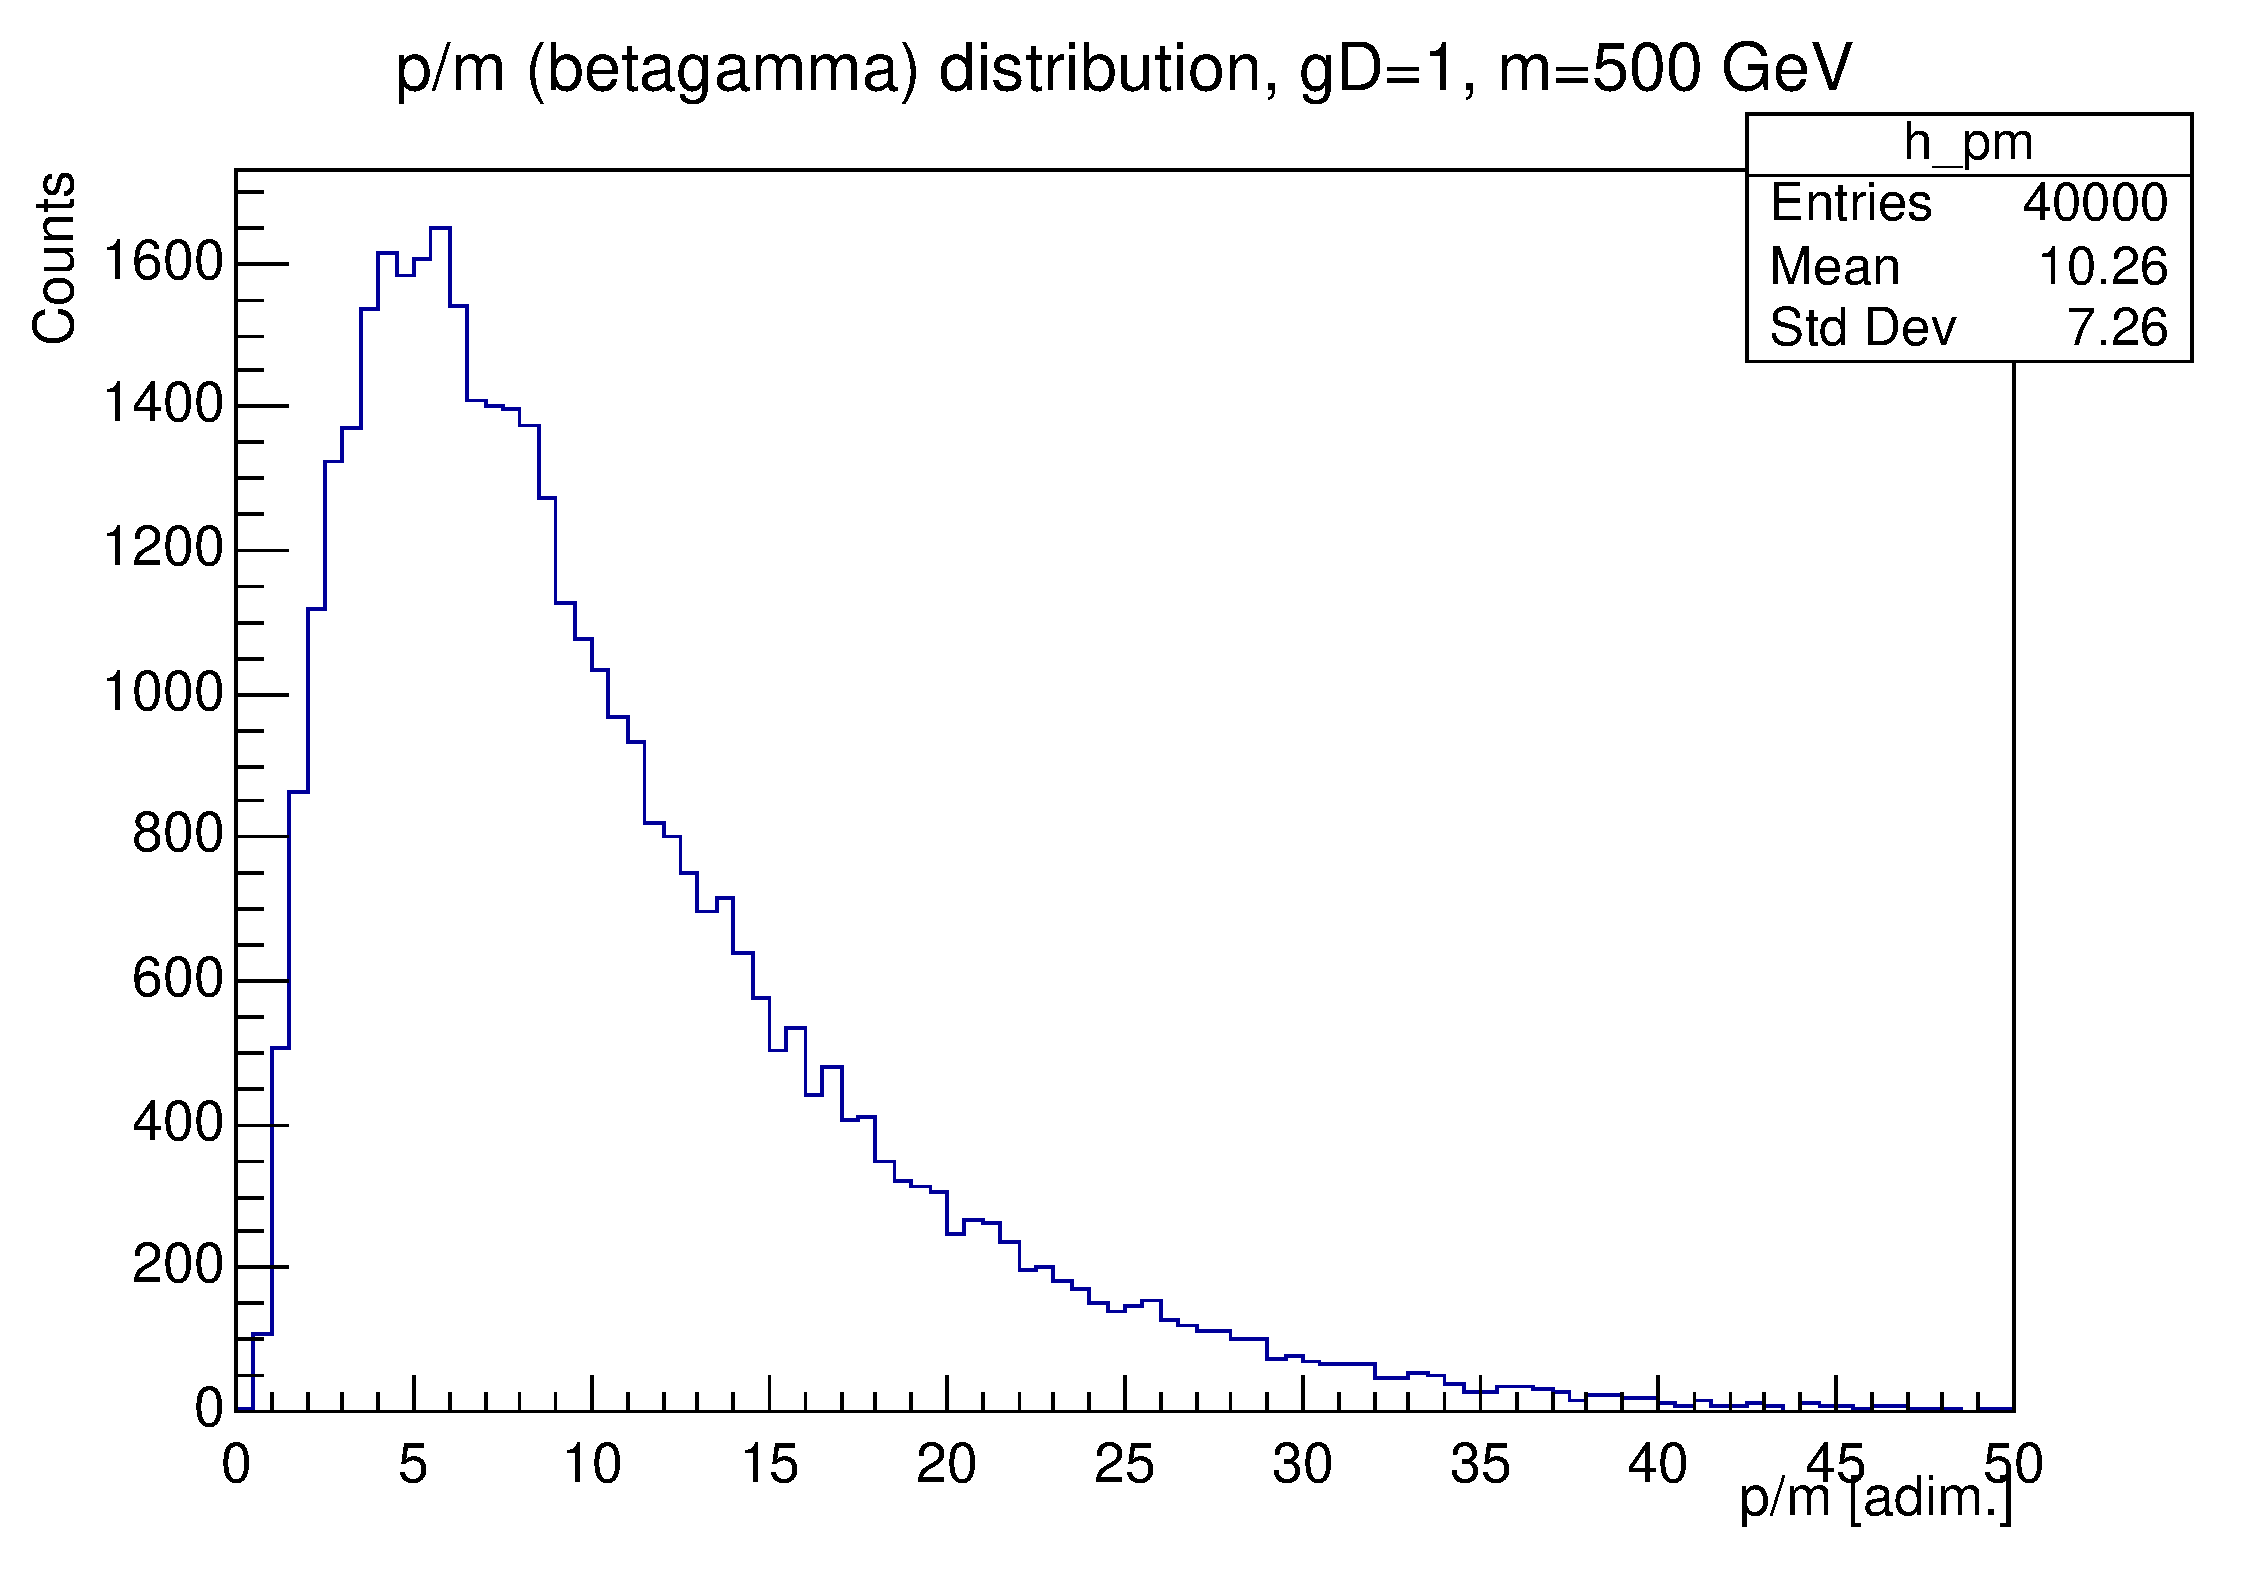
\includegraphics[width=\textwidth]{1.pdf}
        \caption{$m = 500$ GeV, $g = 1g_D$}
        \label{fig:bg_1g_500}
    \end{subfigure}
    \hfill
    \begin{subfigure}[b]{0.48\textwidth}
        \centering
        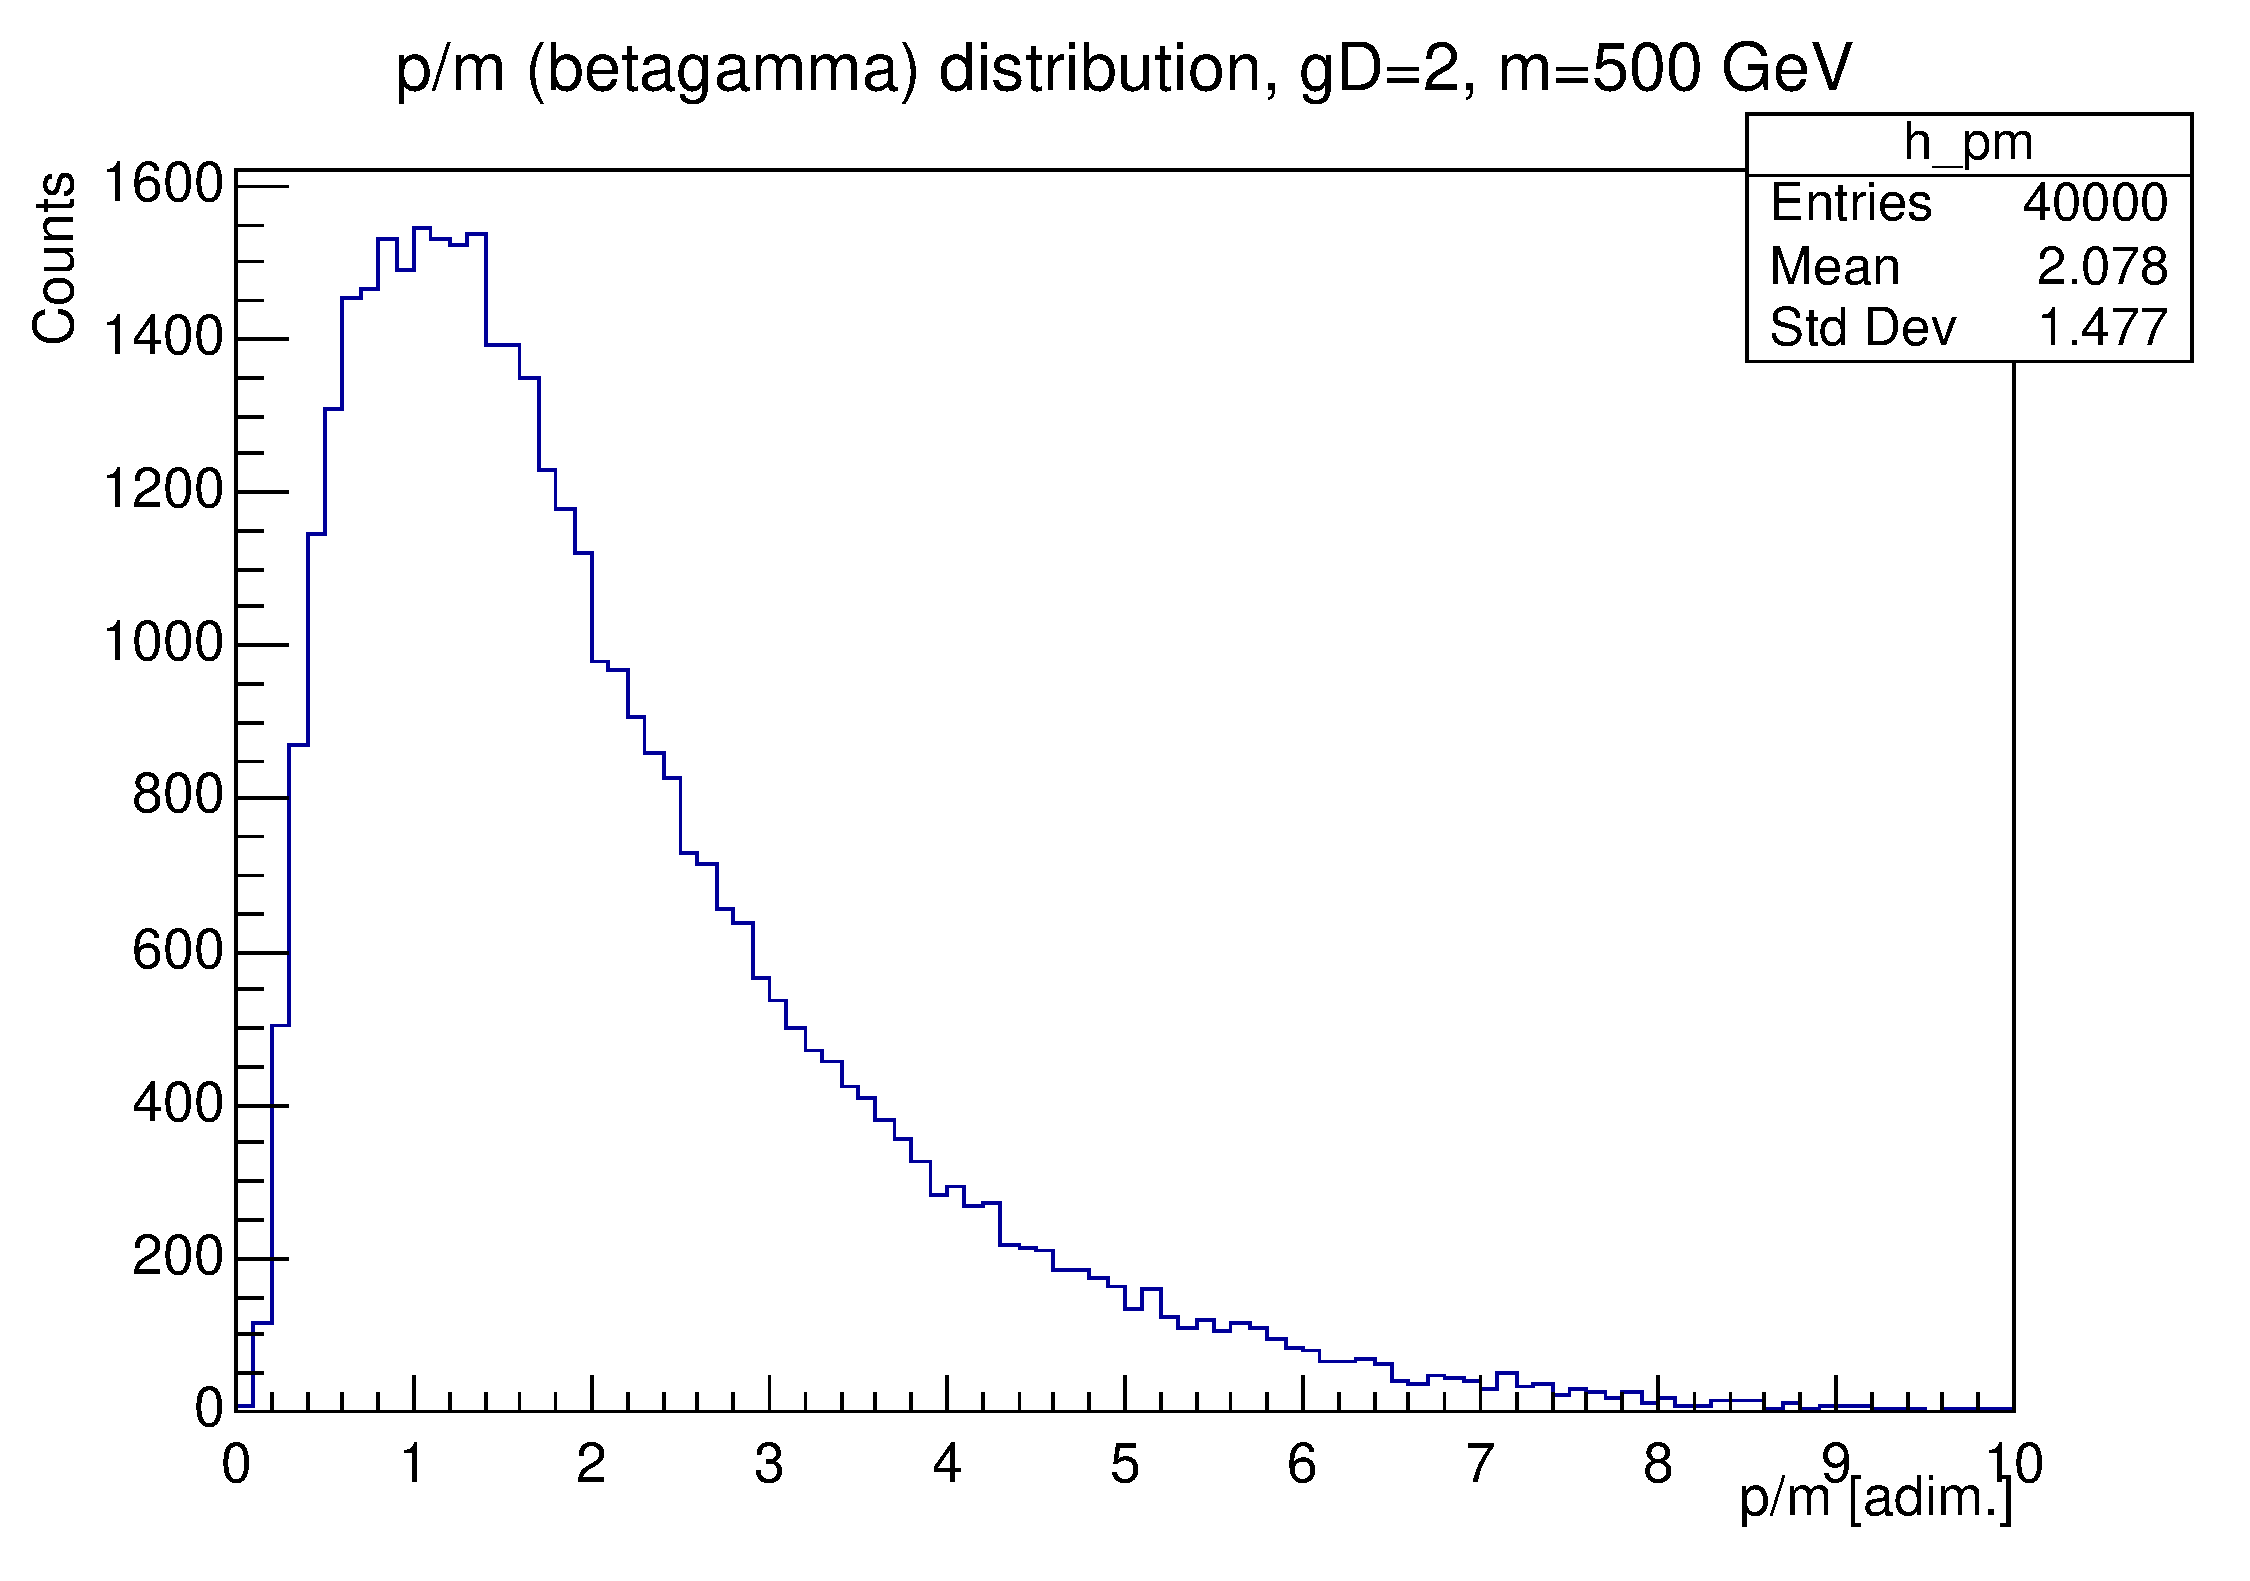
\includegraphics[width=\textwidth]{4.pdf}
        \caption{$m = 500$ GeV, $g = 2g_D$}
        \label{fig:bg_2g_500}
    \end{subfigure}
    
    \vspace{0.5cm} % Vertical spacing between rows
    
    % Row 2: m = 1000 GeV
    \begin{subfigure}[b]{0.48\textwidth}
        \centering
        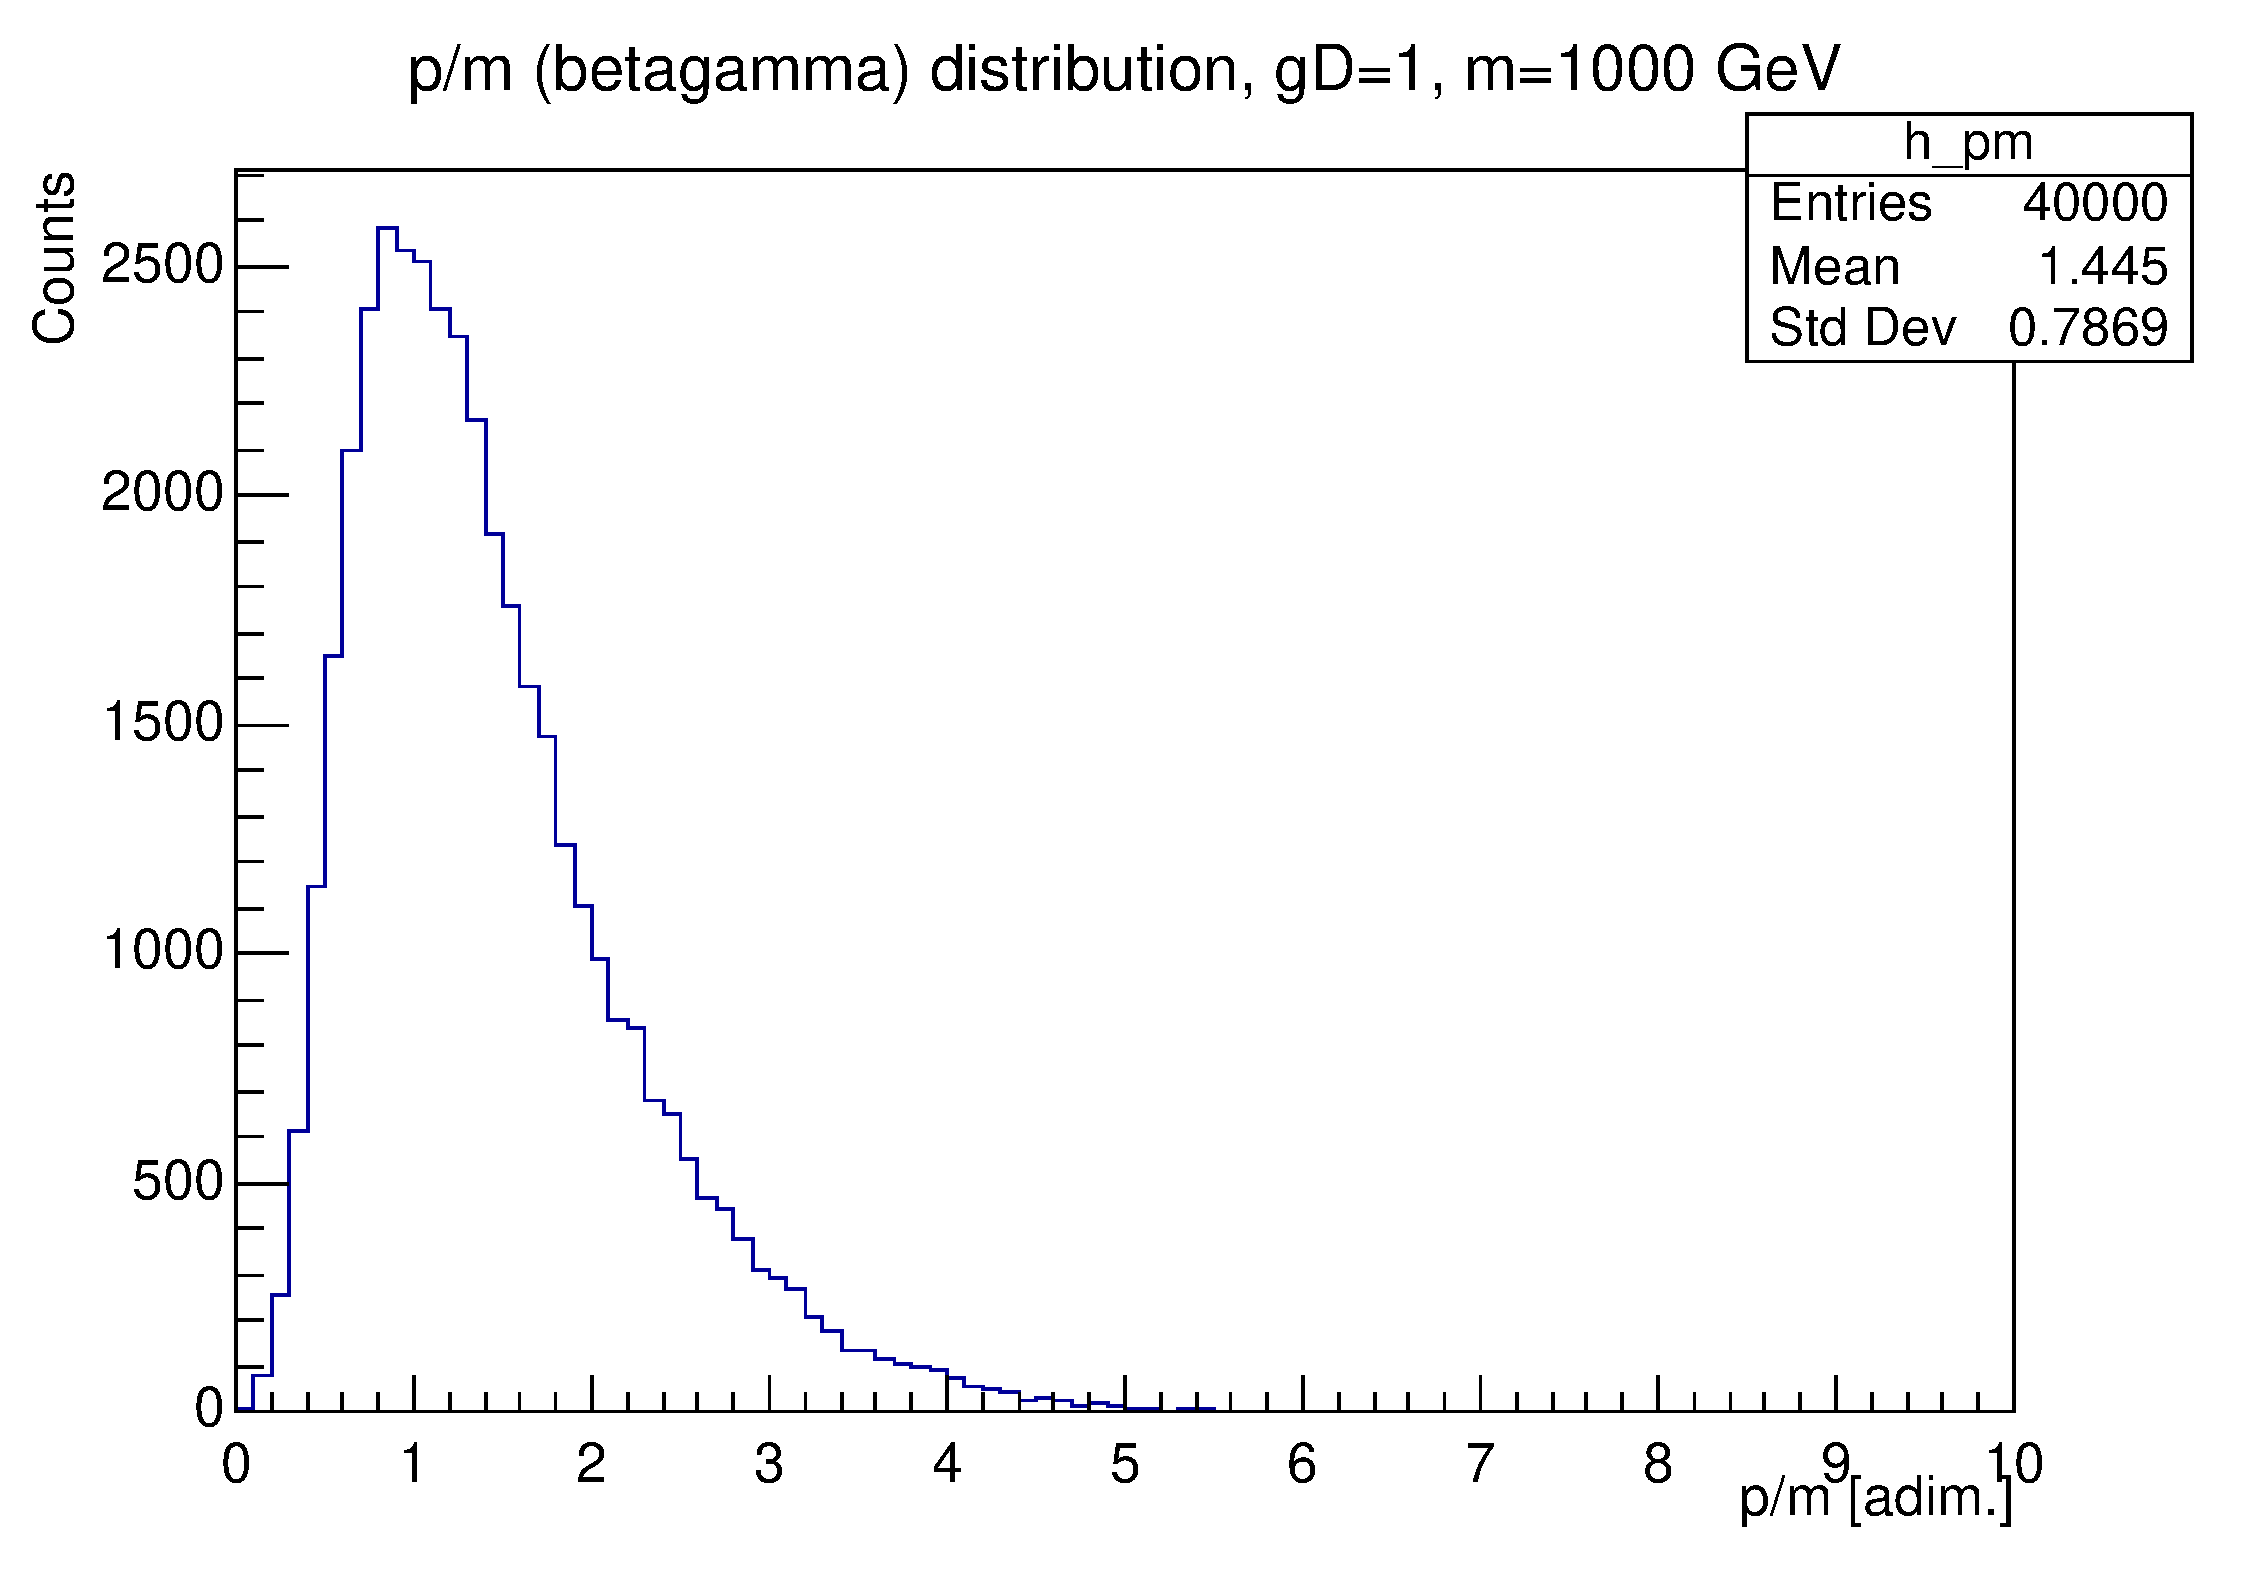
\includegraphics[width=\textwidth]{2.pdf}
        \caption{$m = 1000$ GeV, $g = 1g_D$}
        \label{fig:bg_1g_1000}
    \end{subfigure}
    \hfill
    \begin{subfigure}[b]{0.48\textwidth}
        \centering
        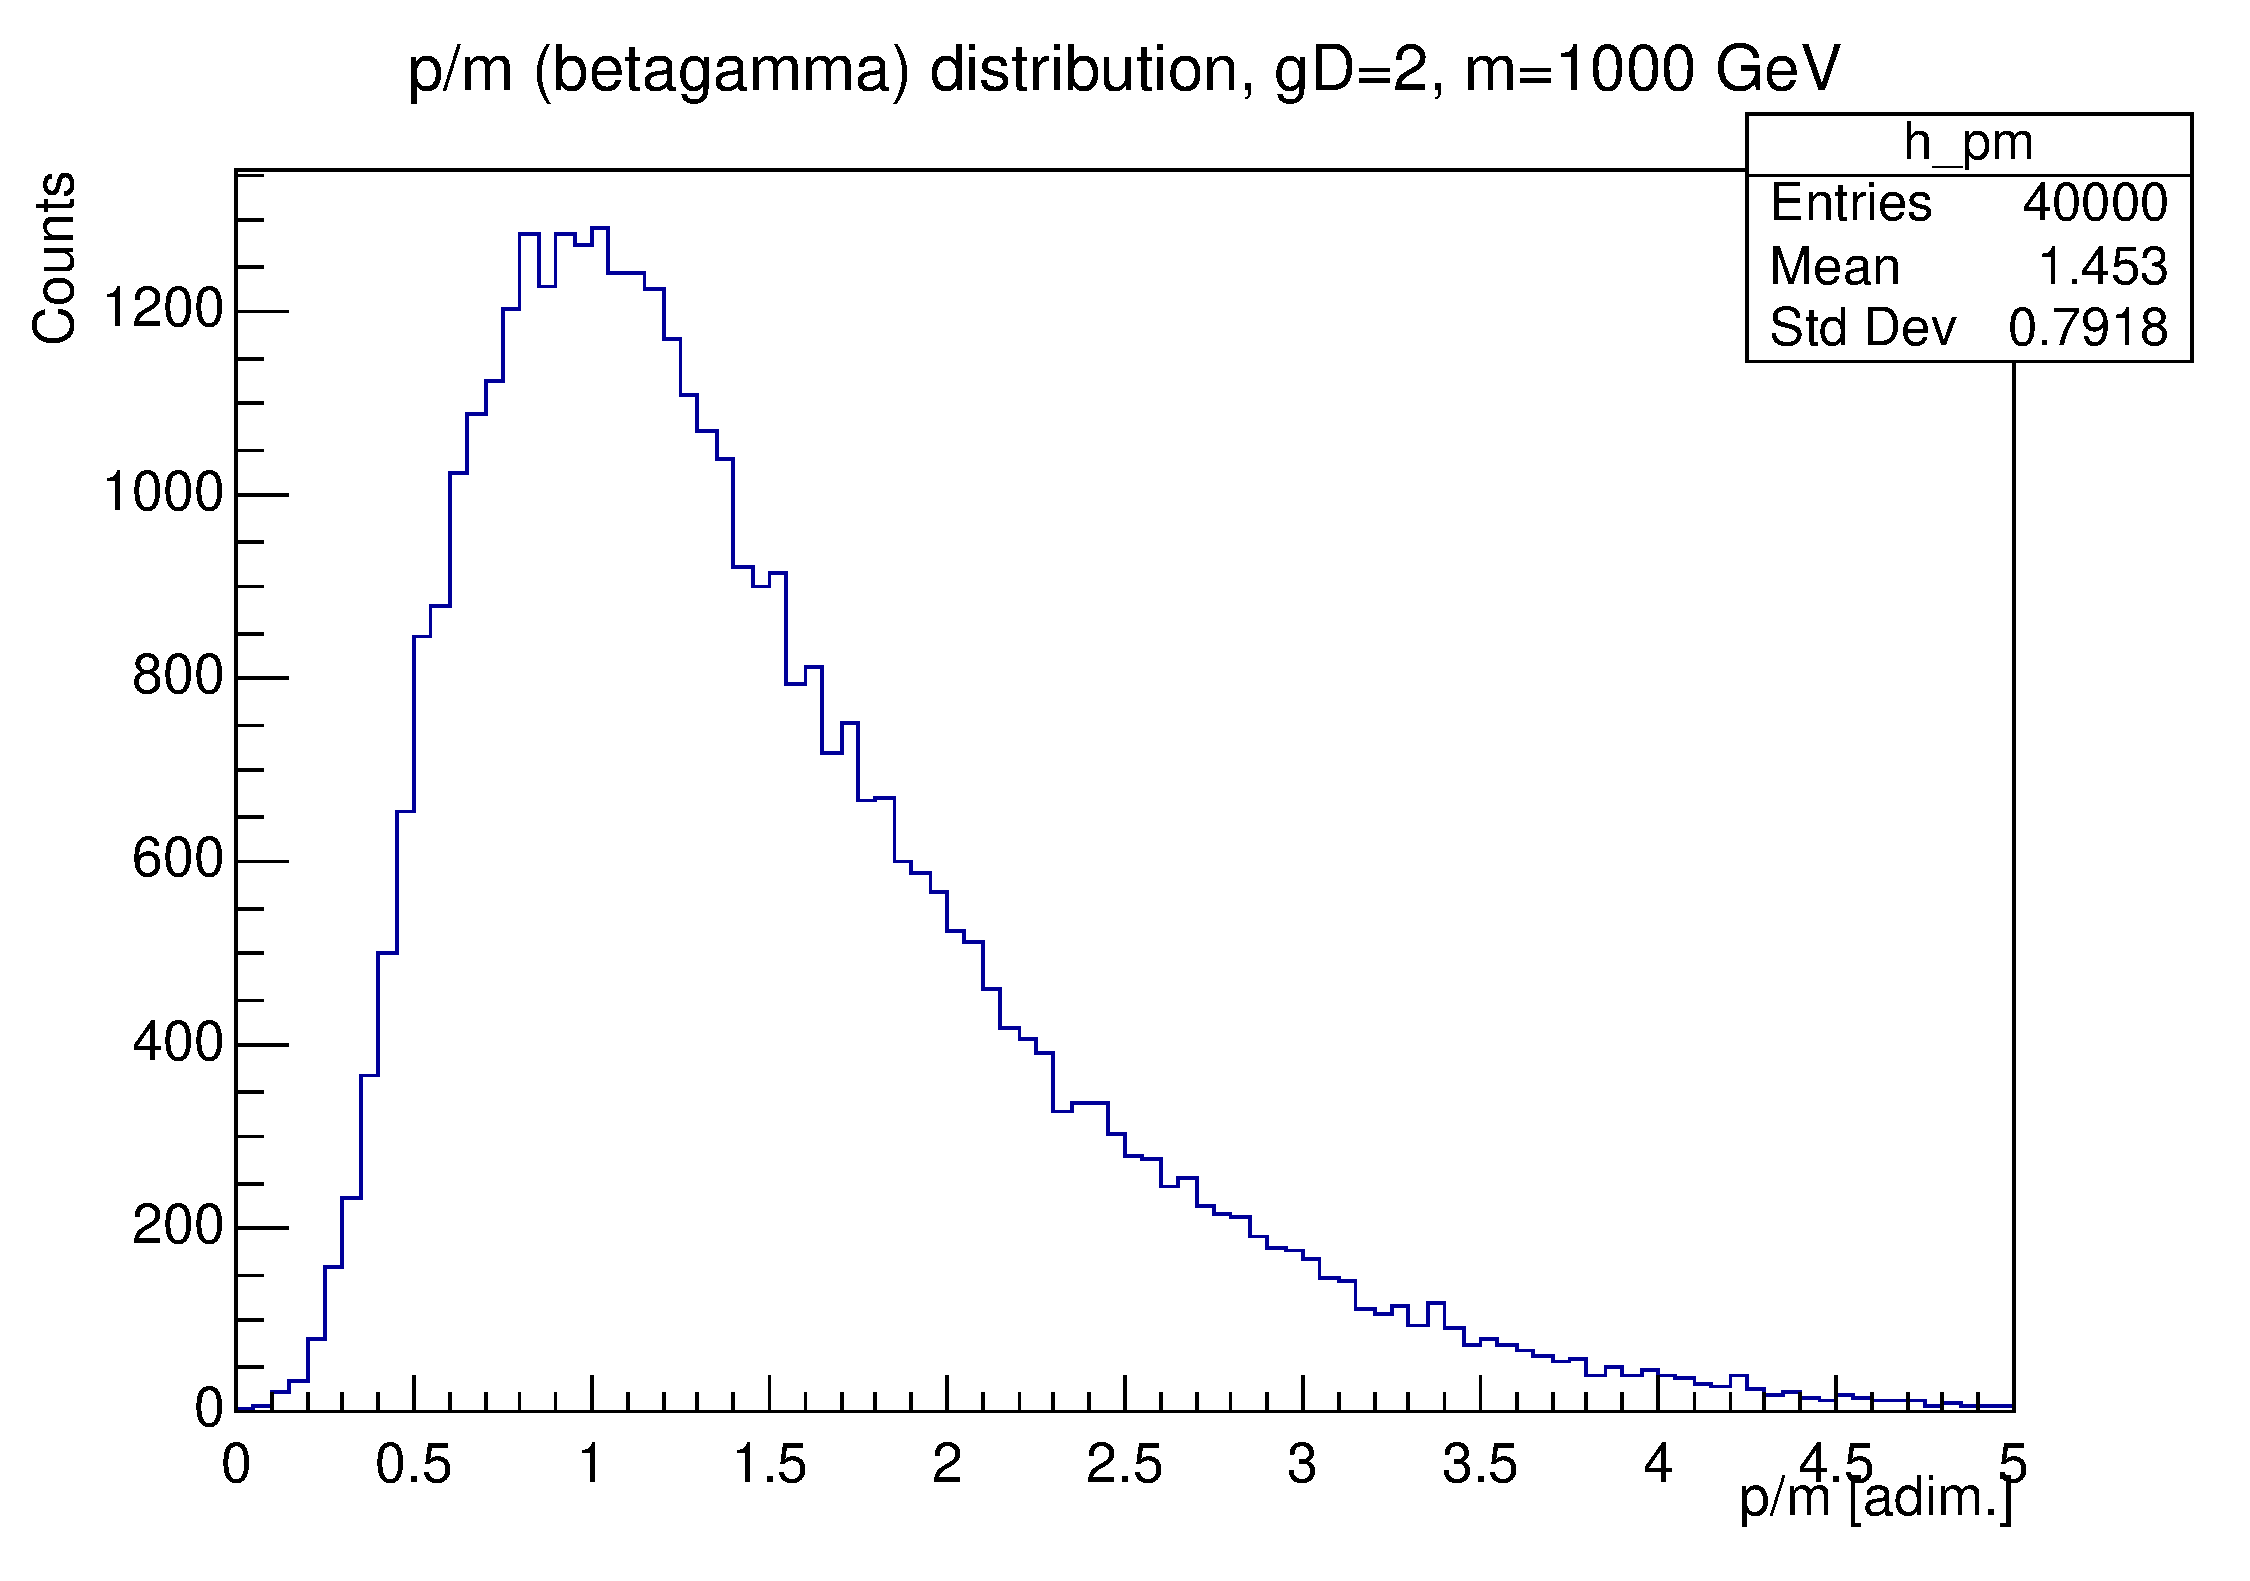
\includegraphics[width=\textwidth]{5.pdf}
        \caption{$m = 1000$ GeV, $g = 2g_D$}
        \label{fig:bg_2g_1000}
    \end{subfigure}
    
    \vspace{0.5cm} % Vertical spacing between rows
    
    % Row 3: m = 1500 GeV
    \begin{subfigure}[b]{0.48\textwidth}
        \centering
        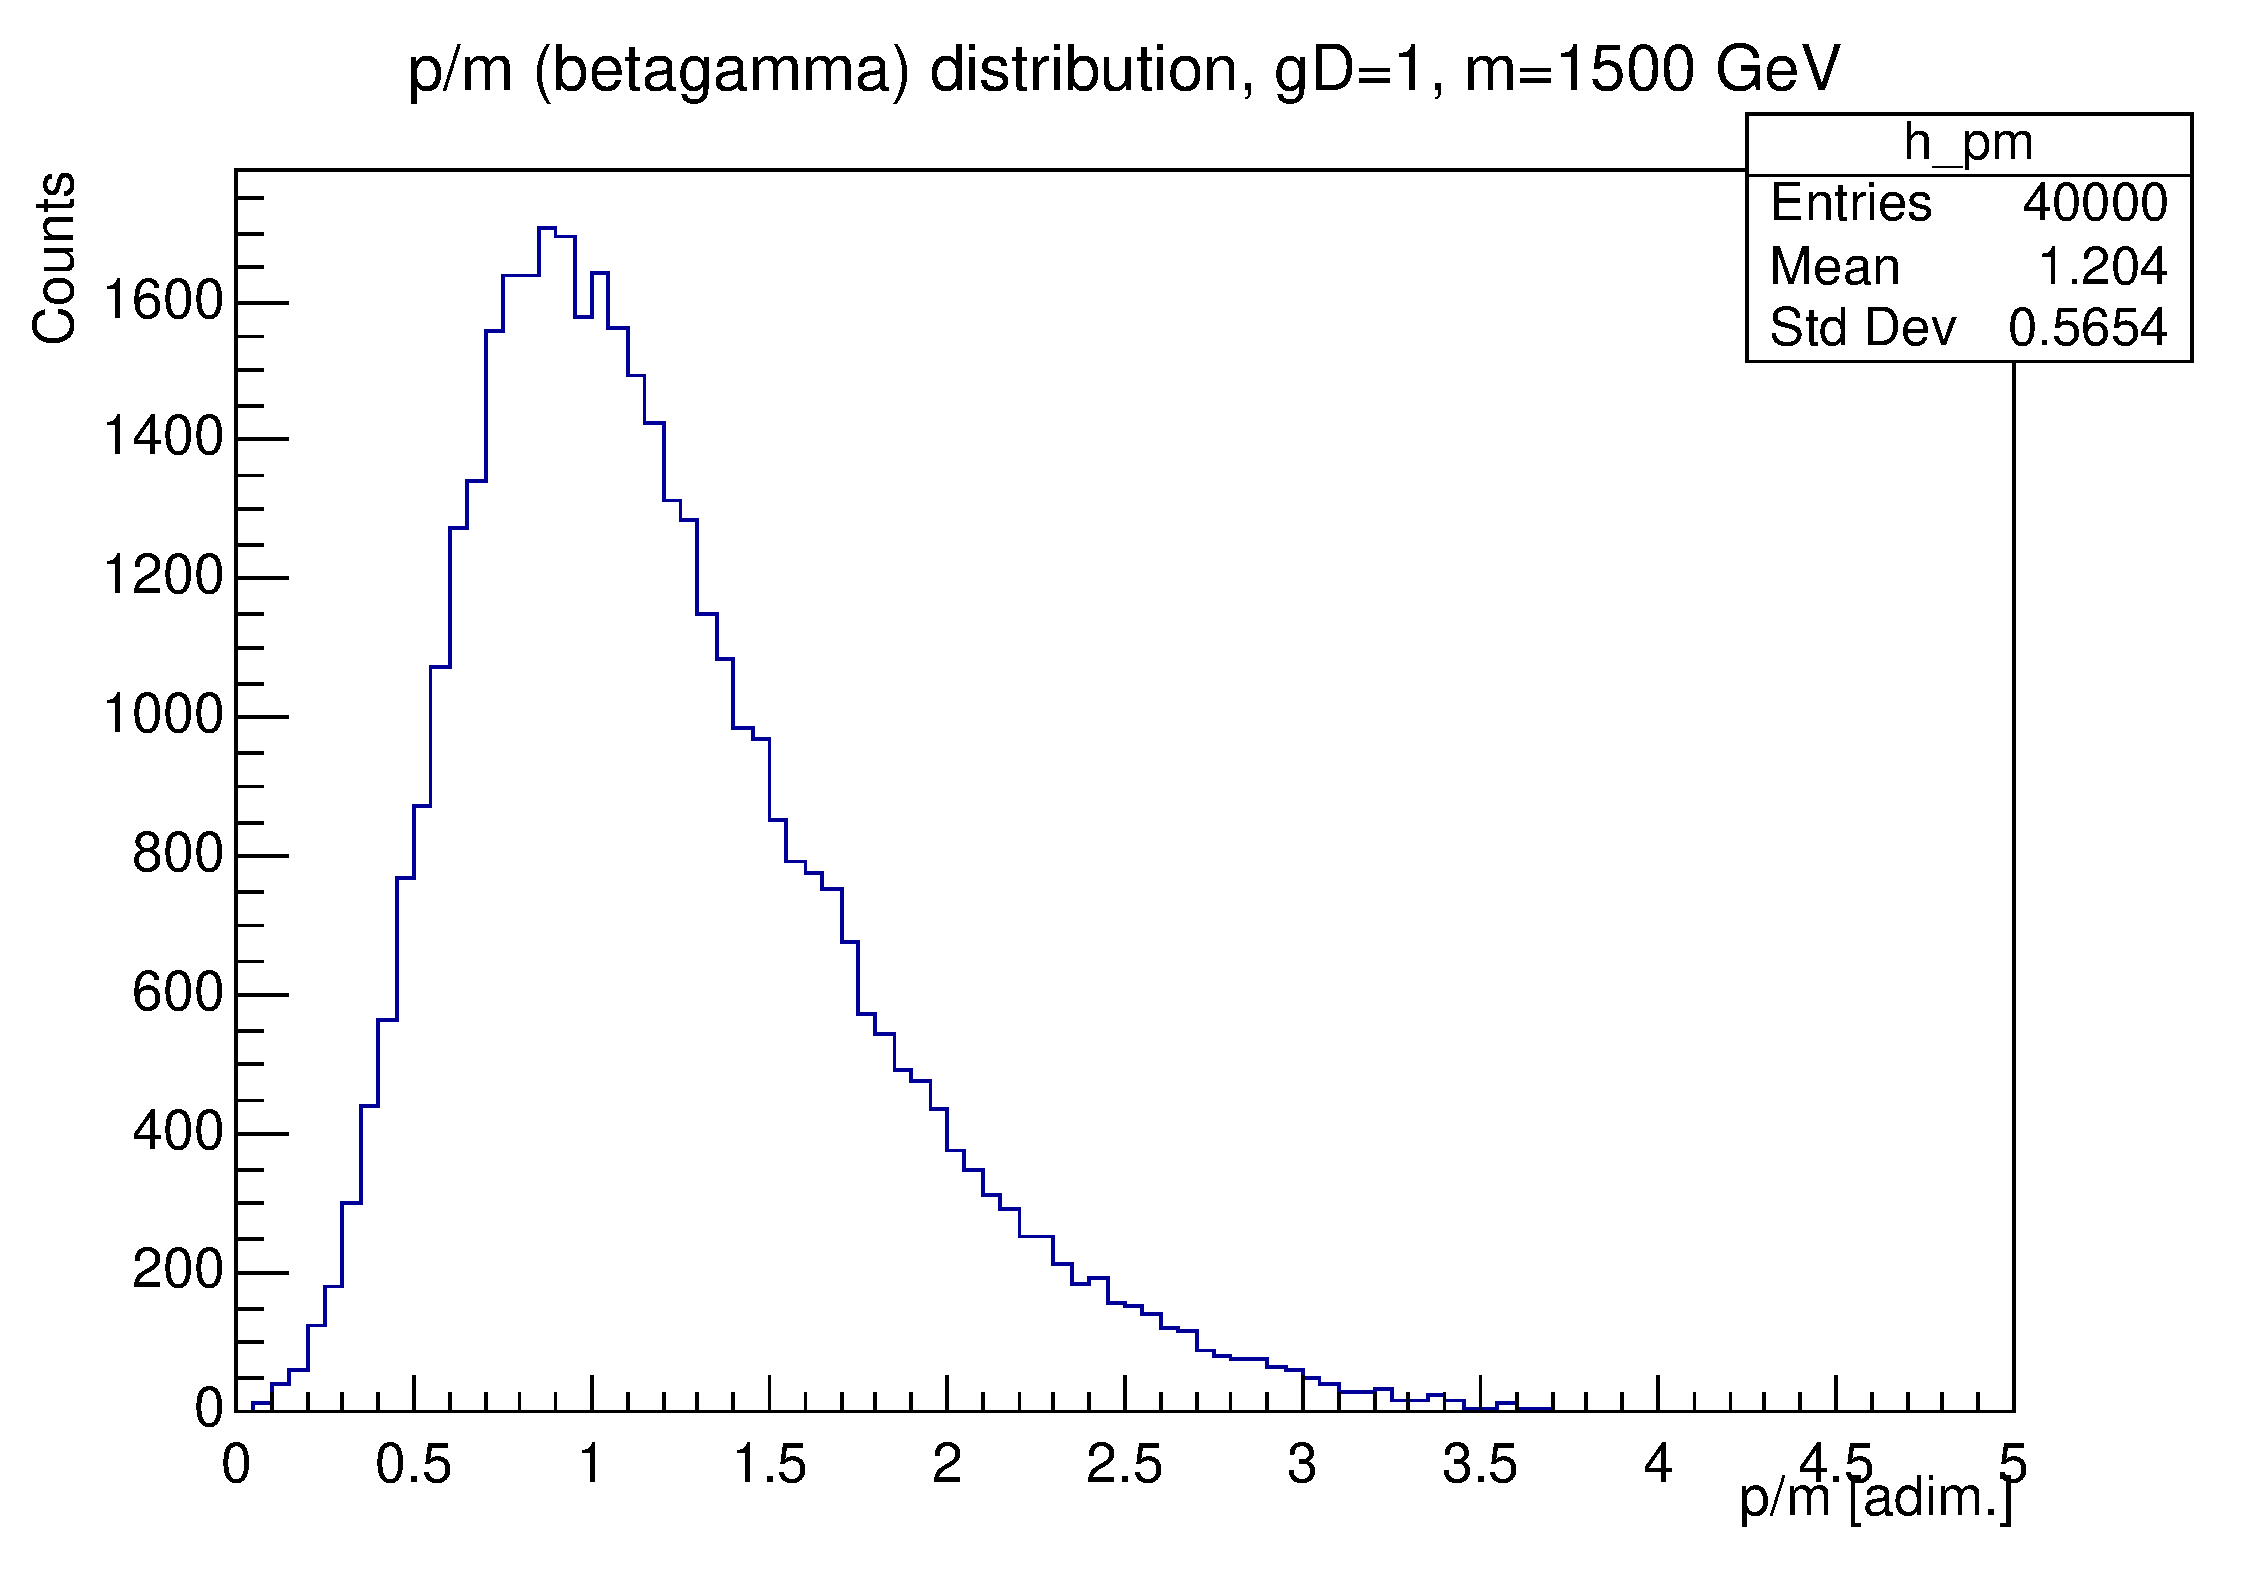
\includegraphics[width=\textwidth]{3.pdf}
        \caption{$m = 1500$ GeV, $g = 1g_D$}
        \label{fig:bg_1g_1500}
    \end{subfigure}
    \hfill
    \begin{subfigure}[b]{0.48\textwidth}
        \centering
        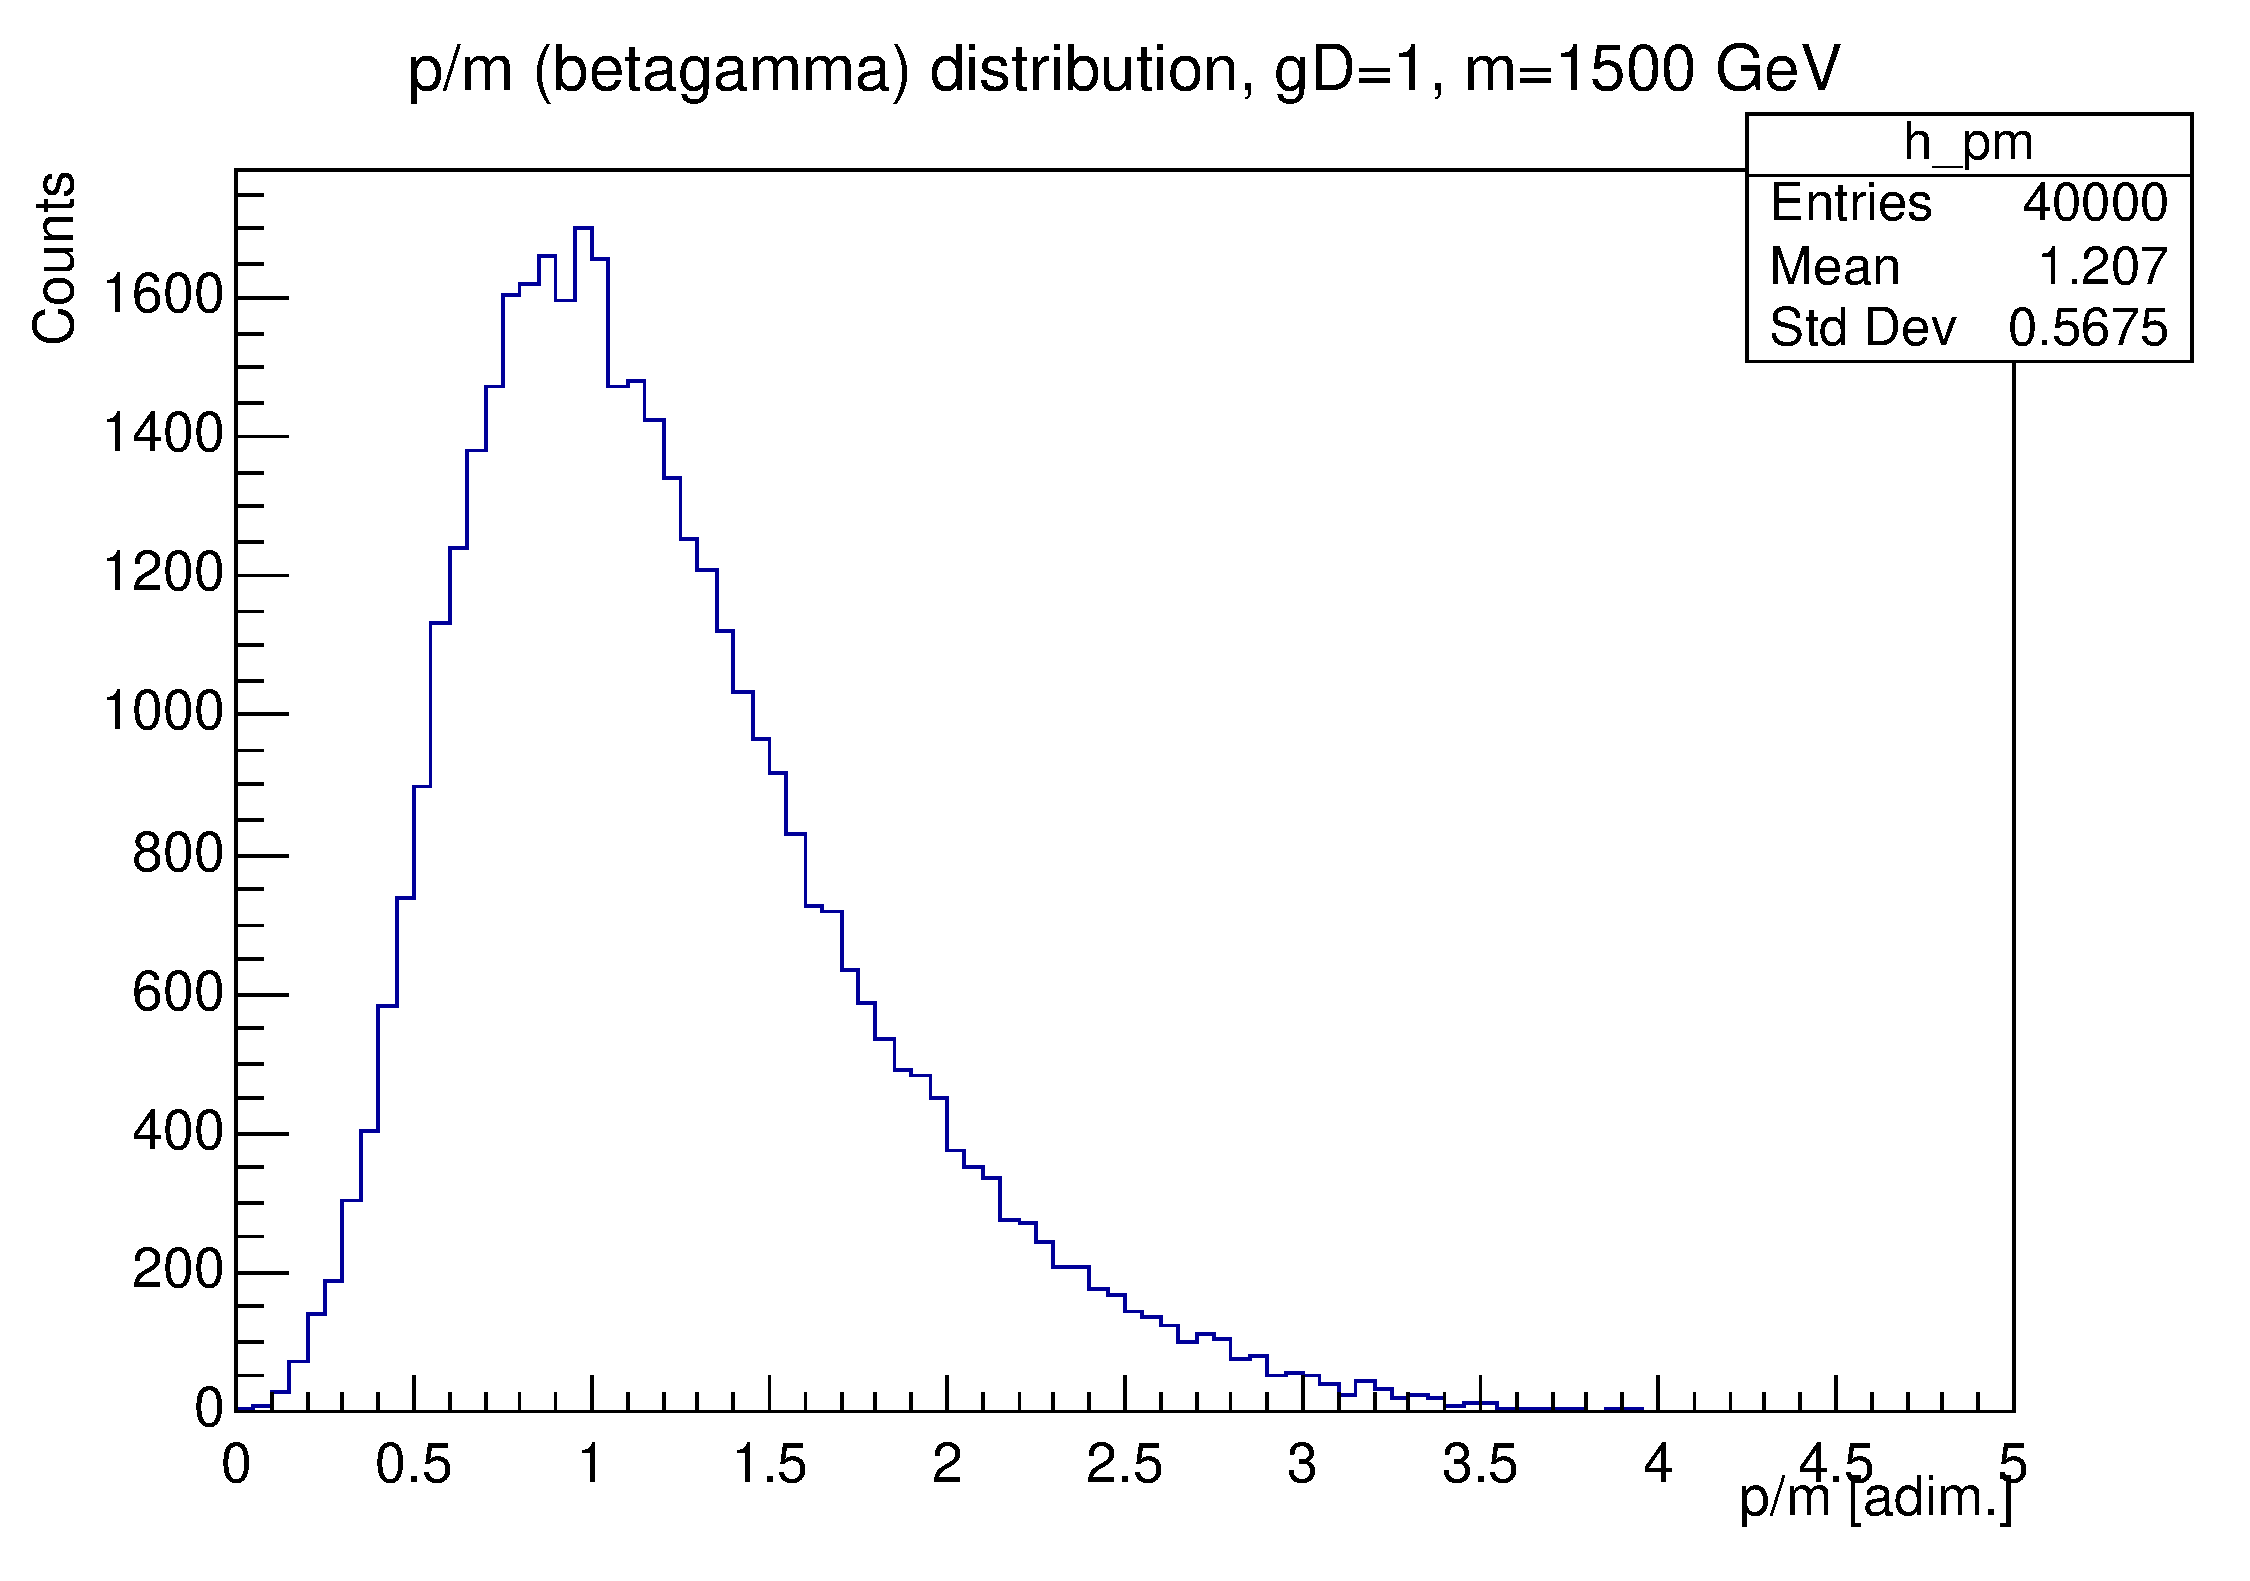
\includegraphics[width=\textwidth]{6.pdf}
        \caption{$m = 1500$ GeV, $g = 2g_D$}
        \label{fig:bg_2g_1500}
    \end{subfigure}
    
    \caption{Distribuciones simuladas de $\beta\gamma$ ($p/m$) para monopolos magnéticos producidos a través del mecanismo de DY. La columna izquierda corresponde a una carga magnética fundamental de $1g_D$, mientras que la columna derecha corresponde a $2g_D$. Las filas representan diferentes valores de masa para el monopolo: 500 GeV, 1000 GeV y 1500 GeV, ilustrando la supresión por espacio de fases y la dinámica cerca del umbral de producción.}
    \label{fig:betagamma_distributions}
\end{figure}



% -------------------------------------------------------------
% SECCIÓN 3: Opinión personal
% -------------------------------------------------------------
\section{Opinión personal}
Considero que esta estancia de investigación ha sido una experiencia sumamente enriquecedora. Los monopolos magnéticos han suscitado mi interés desde el inicio de mis estudios de grado, por lo que he valorado enormemente la oportunidad de profundizar en su estudio, abordándolos de manera exhaustiva tanto desde una perspectiva teórica como experimental.

Durante mi integración en el grupo AITANA, tuve la oportunidad de asistir a las reuniones mensuales del equipo, en las cuales los investigadores más jóvenes (estudiantes de doctorado e investigadores júnior) expusieron los avances de sus respectivos proyectos. Estas sesiones resultaron de gran valor formativo, permitiéndome entrar en contacto con temáticas de gran relevancia actual, tales como las mediciones de materia oscura y el entrelazamiento cuántico en desintegraciones.  En particular, me ha sorprendido gratamente observar las diferencias en el uso de la terminología y las diferentes convenciones a la hora de presentar resultados con respecto la física teórica. 

En conclusión, más allá de los conocimientos técnicos adquiridos, de esta estancia extraigo una lección fundamental: la física teórica y la experimental son disciplinas inseparables, pues ambas se retroalimentan continuamente para lograr comprender las cuestiones más profundas de la naturaleza. En esta sinergia, las simulaciones actúan como un puente crucial entre las dos, guiando y optimizando el desarrollo de las investigaciones experimentales.

% -------------------------------------------------------------
% SECCIÓN 4: Bibliografía
% -------------------------------------------------------------
\small
\begin{thebibliography}{9}
\bibitem{Alwall_2014}
J. Alwall et al.,
\emph{The automated computation of tree-level and next-to-leading order differential cross sections, and their matching to parton shower simulations},
Journal of High Energy Physics \textbf{2014}, no. 7 (2014).

\bibitem{Baines2018}
S. Baines et al., \emph{Monopole production via photon fusion and Drell-Yan processes: MADGRAPH implementation and perturbativity via velocity-dependent coupling and magnetic moment as novel features}, \emph{Eur. Phys. J. C} {\bf 78} (2018) 996.

\bibitem{Dirac1931}
P. A. M. Dirac, \emph{Quantised singularities in the electromagnetic field}, \emph{Proc. Roy. Soc. Lond. A} {\bf 133} (1931) 60-72.

\bibitem{AITANA}
\textit{Grupo AITANA}. URL: \url{https://aitanatop.ific.uv.es/aitanatop/} (Consultado el 1 de junio de 2026).

\bibitem{mitsou2026magneticmonopolesdirac}
Vasiliki A. Mitsou, \emph{Magnetic Monopoles -- From Dirac to the Large Hadron Collider}, arxiv:2605.02869.

\bibitem{2016}
The MoEDAL Collaboration, \emph{Search for magnetic monopoles with the MoEDAL prototype trapping detector in 8 TeV proton-proton collisions at the LHC}, \emph{JHEP} {\bf 2016} (2016) 067.

\bibitem{MoEDAL2017}
The MoEDAL Collaboration, \emph{Search for magnetic monopoles with the MoEDAL forward trapping detector in 13 TeV proton-proton collisions at the LHC}, \emph{Phys. Rev. Lett.} {\bf 118} (2017) 061801.

\bibitem{MoEDAL2022}
The MoEDAL Collaboration, \emph{First search for magnetic monopoles through the Schwinger mechanism}, \emph{Nature} {\bf 602} (2022) 63.

\bibitem{Polyakov1974}
A. M. Polyakov, \emph{Particle spectrum in quantum field theory}, \emph{JETP Lett.} {\bf 20} (1974) 194-195.

\bibitem{doi:10.1126/science.165.3895.757}
Julian Schwinger, \emph{A Magnetic Model of Matter}, \emph{Science} {\bf 165} (1969) 757-761.

\bibitem{tHooft1974}
G. 't Hooft, \emph{Magnetic monopoles in unified gauge theories}, \emph{Nucl. Phys. B} {\bf 79} (1974) 276-284.

\end{thebibliography}

\end{document}